\documentclass[article,colorback,accentcolor=tud4c]{tudreport}
% \usepackage{ngerman}

\usepackage[stable]{footmisc}
\usepackage{hyperref}

\usepackage{longtable}
\usepackage{multirow}
\usepackage{booktabs}

% \hypersetup{%
%   pdftitle={Eclipse Plug-in Development},
%   pdfauthor={Leo Roos},
%   pdfsubject={Beispieltext},
%   pdfview=FitH,
%   pdfstartview=FitV
% }

% \setcounter{seclinedepth}{1}
% 
% %%% Zum Tester der Marginalien %%%
%   \newif\ifTUDmargin\TUDmarginfalse
%   %%% Wird der Folgende Zeile einkommentiert,
%   %%% werden Marginalien gesetzt.
%   % \TUDmargintrue
%   \ifTUDmargin\makeatletter
%     \TUD@setmarginpar{2}
%   \makeatother\fi
% %%% ENDE: Zum Tester der Marginalien %%%
% 
% \newlength{\longtablewidth}
% \setlength{\longtablewidth}{0.7\linewidth}
% \addtolength{\longtablewidth}{-\marginparsep}
% \addtolength{\longtablewidth}{-\marginparwidth}


% \settitlepicture{tudreport-pic}
% \printpicturesize

\newcommand\tiger{%
  \textsc{TigersEye}
}


\newcommand\versionnum{%
  \texttt{0.0.1}
}

\newcommand\version{%
  v. \versionnum
}

\title{\tiger \version \\User Manual}
\subtitle{Leo Roos}
\subsubtitle{\href{mailto:leo\_roos@rbg.informatik.tu-darmstadt.de}{leo\_roos@rbg.informatik.tu-darmstadt.de}}
\institution{Department of Computer Science\\Advisor: Tom Dinkelaker}

\begin{document}
  \maketitle

  \tableofcontents

  \section{Introduction}
  The \tiger Eclipse Plug-in is an IDE that strives to support easy creation of EDSLs. This guide describes how to install  \tiger for development, the currently implemented features and shows on some examples how to create and install a new language.
  \tiger has been previously known as \texttt{Popart}, which has been developed by Yevgen Fanshil[Reference1], Leonid Melnyk [Reference1], Thorsten Peter [Ref2], David Marx[Ref2], Kamil Erhard [?] and Tom Dinkelaker[Langs?]. The used examples are adjusted versions of their prior work.  

  \newpage

  \section{Installation for Development}
	
	The \tiger plug-in itself consists of multiple separate plug-ins and has further dependencies to other plug-ins and libraries. It uses classes and extensions from the Groovy Plug-in and  Eclpse's JDT plug-ins, makes some use of different \texttt{apache.commons} libraries and uses further libraries to process code. It's core dependency is the used preprocessor \texttt{parlex}. Listing \ref{lst:dependencies} shows the necessary plug-ins and the required version if any.
	
	
	\begin{table}
	\centering
	  \begin{tabular}{|l|l|p{.4\textwidth}|}
		\hline
		Plug-in name & Version & Description\\ \hline	
		de.tud.stg.tigerseye.eclipse.core & \versionnum & Core functionality.\\
		de.tud.stg.tigerseye.eclipse.ui& \versionnum & User Interface functionality.\\
		de.tud.stg.tigerseye & \versionnum & (Re)Exports commonly used libraries and plug-ins.\\
		Groovy Eclipse Feature & 2.1.1 & Groovy Eclipse Plug-ins with version that is known to be compatible.\\
		org.apache.commons.collections & - & Apache utility classes for collections.\\
		org.apache.commons.io & - & Apache IO utility classes.\\
		org.apache.commons.lang& - & Apache general language utility classes.\\
		org.apache.log4j & [1.2 - 1.3) & Employed logging framework.\\
		parlex & - & Preprocessor, performing the transformations. \\
		slf4j-log4j12 & - & Employed logging facade with log4j binding.\\
		\hline
	  \end{tabular}
	  \caption{Necessary Plug-ins}\label{lst:dependencies}\label{lst:dependencies}
	\end{table}
	

	Once all the necessary plug-ins have been installed the \tiger plug-in can be started using the predefined \texttt{Tigerseye\_IDE} launch, which is located in the core plug-in. 
	It is possible that depending on the used operating system this launch configuration has to be adjusted. Alternatively one can start a new Eclipse Plug-in configuration with all available plug-ins active.
	

  \section{Features}

	The current version of \tiger provides the fundamental functaionlities in order to be able to use it as a language workbench. New languages can easily be created and deployed. After a restart they can be used in projects that have the \tiger nature. A \tiger nature can easily be added and removed via a popup menu. The installed DSLs can be configured through the preference pages, as well as the employed transformations. The \tiger editor is an extended version of the Groovy editor and provides keyword coloring for keywords of installed and activated DSLs.
	
	\subsection{Preferences}
	The prefrence pages are an important part of \tiger, since they provide the configuration of registered DSLs. In the main prefrence page (Figure \ref{fig:prefs_main}) the output source folder can be adjusted.
	
	Registered languages can be configured on the languages preference page (Figure \ref{fig:prefs_languages}). DSLs have to be set into activated state in order to use them.	
	The extensions, that indicate which concrete DSL class is responsible for which files of the according extension can be adjusted in the \texttt{Extensions} column. When a DSL is selected its keywords are shown below in the \textit{Declared Keywords of Selected DSL} dialog.
	
	The transformations preference page provides the adjustment of used transformations for the specified resource or DSL (Figure \ref{fig:prefs_transformations}). For each resource and DSL different transformations might be provided. These can be configured using the \texttt{Select Transformations} dialog (Figure \ref{fig:prefs_transformations_selected}). The dialog also shows additional informations about the currently selected transformation in a tray window that can be opened clicking on the additinal information button (Figure \ref{fig:additional_information_button}). The \tiger editor provides keyword coloring for active DSLs. The colors can be configured using the Tigerseye Editor preference page (see Figure \ref{fig:prefs_editor}), where every DSL can be configured seperately and the general keyword coloring can be activated or deactivated.
	
	\begin{figure}
	  \centering
	  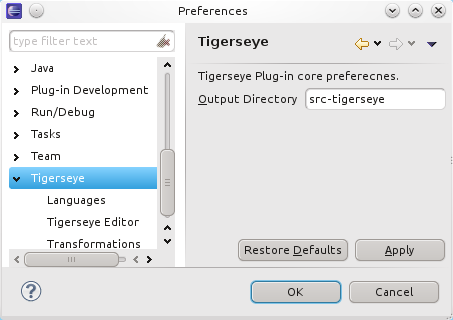
\includegraphics[scale=.5,keepaspectratio=true]{./pics/preferences_main.png}
	  \caption{Tigerseye Main Preference Page}
	  \label{fig:prefs_main}
	\end{figure}

	\begin{figure}
	  \centering
	  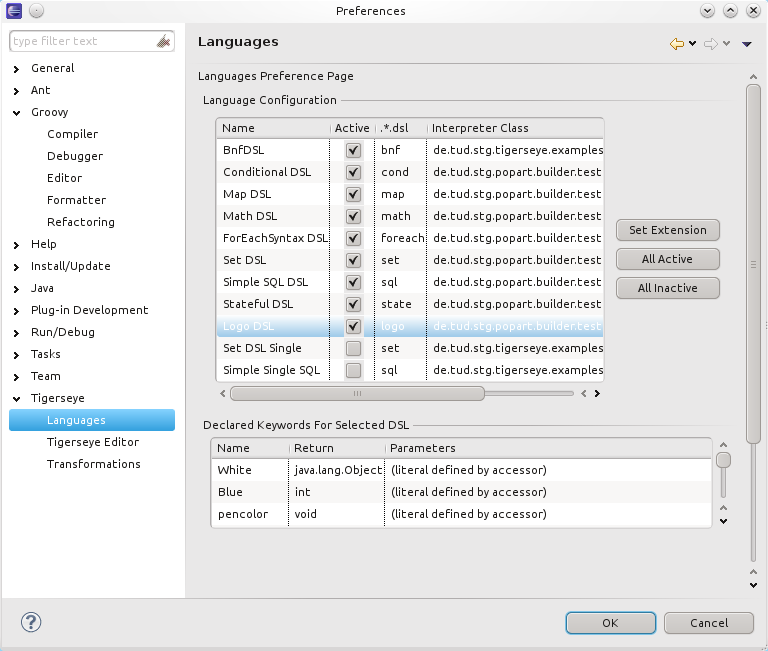
\includegraphics[scale=.5,keepaspectratio=true]{./pics/preferences_languages.png}
	  \caption{Tigerseye Language Configuration Page}
	  \label{fig:prefs_languages}
	\end{figure}

	\begin{figure}
	  \centering
	  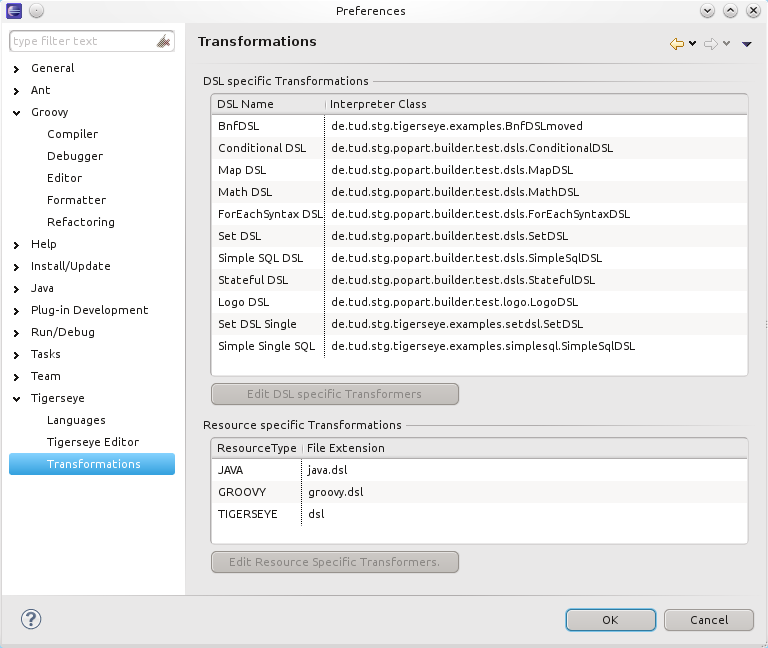
\includegraphics[scale=.5,keepaspectratio=true]{./pics/preferences_transformations.png}
	  \caption{Tigerseye Transformations Preference Page}
	  \label{fig:prefs_transformations}
	\end{figure}

	\begin{figure}
	  \centering
	  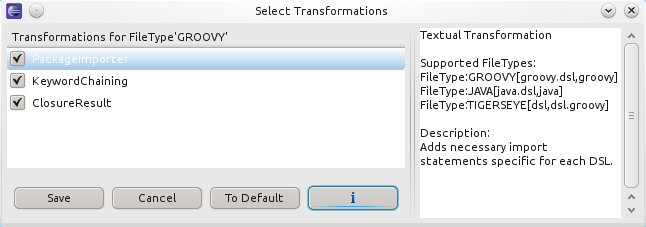
\includegraphics[scale=.5,keepaspectratio=true]{./pics/preferences_transformations_selected.png}
	  \caption{Tigerseye Transformations Configuration}
	  \label{fig:prefs_transformations_selected}
	\end{figure}

	\begin{figure}
	  \centering
	  
\includegraphics{./pics/additional_information_button.png}
	  \caption{Additional Information Button}
	  \label{fig:additional_information_button}
	\end{figure}

	\begin{figure}
	  \centering
	  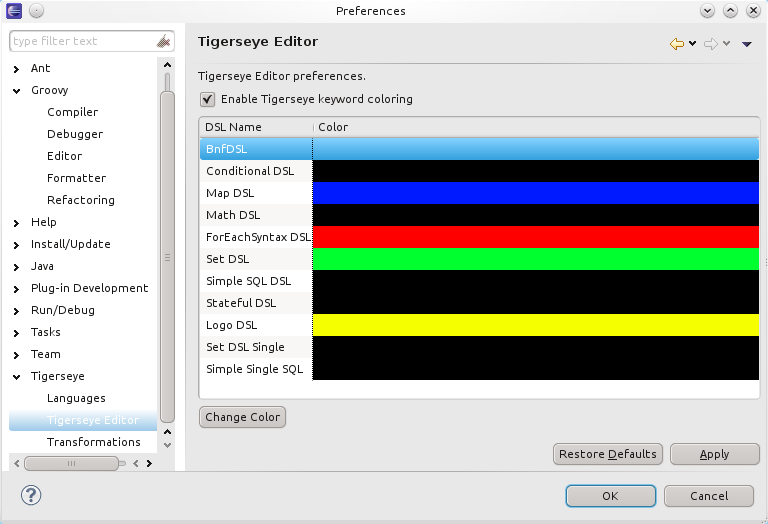
\includegraphics[scale=.5,keepaspectratio=true]{./pics/preferences_editor.png}
	  \caption{Tigerseye Editor Preference Page}
	  \label{fig:prefs_editor}
	\end{figure}

	\subsection{Add and Remove \tiger Nature}
	  \tiger has additional requirements which will be imported when adding the \tiger nature to a project. The project must have at least the Java nature otherwise the transformation to a \tiger project is not possible. Figure \ref{fig:add_tiger_nature} shows the available popup menu to add the \tiger nature to a project. This will do two things. A seperate source folder will be created into which the translated DSL files will be output (here: \texttt{src-tigerseye}) and a new class path container will be added which contains the runtime libraries (\texttt{popartAnnotations.jar, popart.jar, edslNature.jar}) and the libraries of registered DSLs as well as their dependencies. For example \texttt{de.tud.stg.tigerseye.examples.LogoDSL} and \texttt{de.tud.stg.tigerseye.examples.DSLDefinitions}. Additionally the \texttt{GroovyNature} will be added if not already configured.
	
	\begin{figure}
	  \centering
	  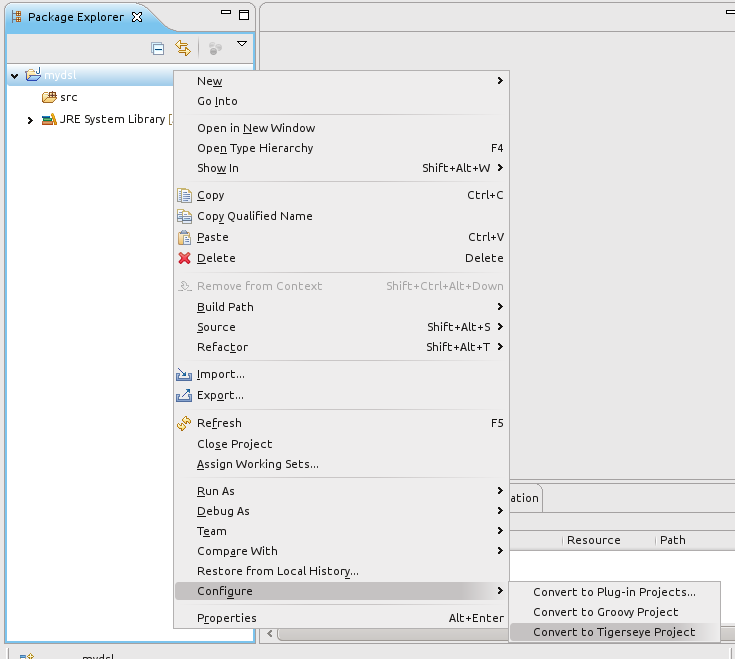
\includegraphics[width=.5\textwidth,keepaspectratio=true]{./pics/convert_to_tigerseye.png}
	  % new_tigesreye_language.png: 525x500 pixel, 93dpi, 14.34x13.66 cm, bb=0 0 406 387
	  \caption{Add the \tiger Nature to a Java Project}
	  \label{fig:add_tiger_nature}
	\end{figure}
	
	\begin{figure}
	  \centering
	  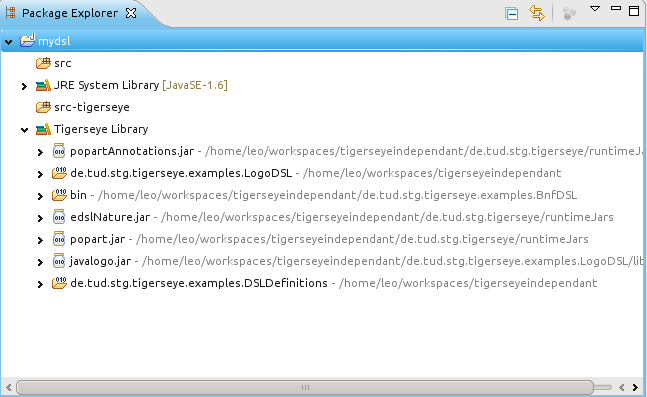
\includegraphics[width=.5\textwidth,keepaspectratio=true]{./pics/tigerseye_dependencies.png}
	  % new_tigesreye_language.png: 525x500 pixel, 93dpi, 14.34x13.66 cm, bb=0 0 406 387
	  \caption{\tiger Dependencies}
	  \label{fig:tiger_added_dependencies}
	\end{figure}
	
	\begin{figure}
	  \centering
	  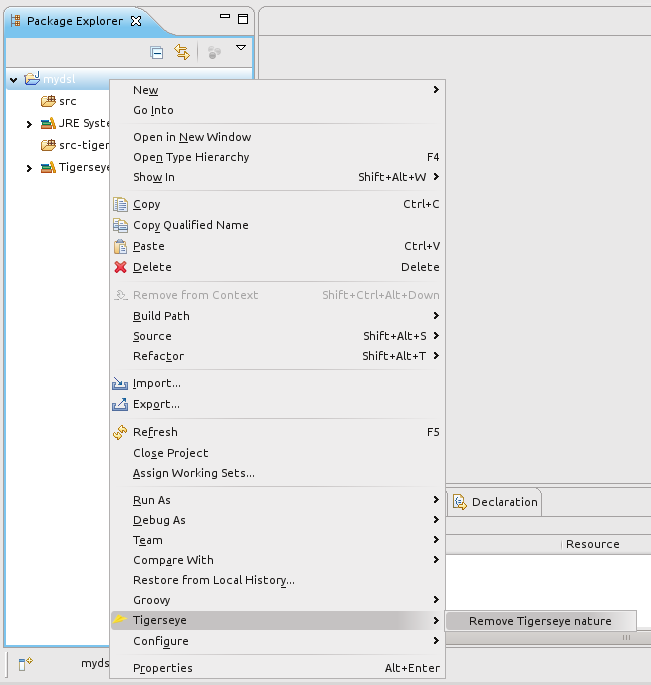
\includegraphics[width=.5\textwidth,keepaspectratio=true]{./pics/remove_tigerseye_nature.png}
	  % new_tigesreye_language.png: 525x500 pixel, 93dpi, 14.34x13.66 cm, bb=0 0 406 387
	  \caption{Remove the \tiger Nature from a Project}
	  \label{fig:remove_tiger_nature}
	\end{figure}
	
	\subsection{\tiger Language Definition Wizard}
	  A new language can be created using the \textit{New Language Wizard}. The Wizard can be accessed via File -> New -> Other (Figure \ref{fig:new_tiger_lang}). Figure \ref{fig:tiger_lang_definition_page1} shows the first page of the Wizard. There the name of the main language class can be defined. As can be seen in the figure the default package is not a valid package for a language defintion since this will cause problems when trying to use the language within a Java class. Figure \ref{fig:tiger_lang_definition_page2} shows the actual language definition page. There the different literals, operations and structured elements can be added. In Section \ref{sec:examples} the usage of the wizard will be showcased.
	
	\begin{figure}
	  \centering
	  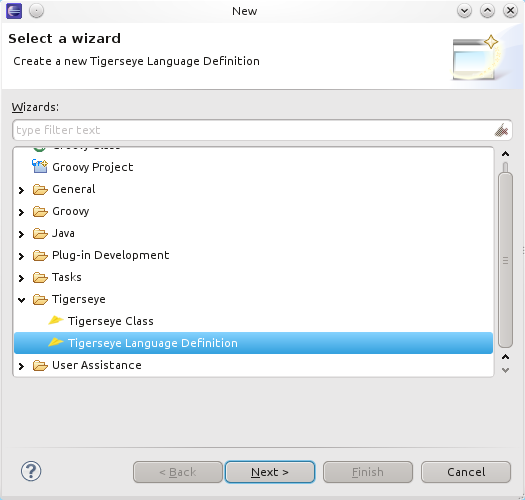
\includegraphics[width=.5\textwidth,keepaspectratio=true]{./pics/new_tigesreye_language.png}
	  \caption{Choosing the New Tigerseye Language Wizard}
	  \label{fig:new_tiger_lang}
	\end{figure}

	\begin{figure}
	  \centering
	  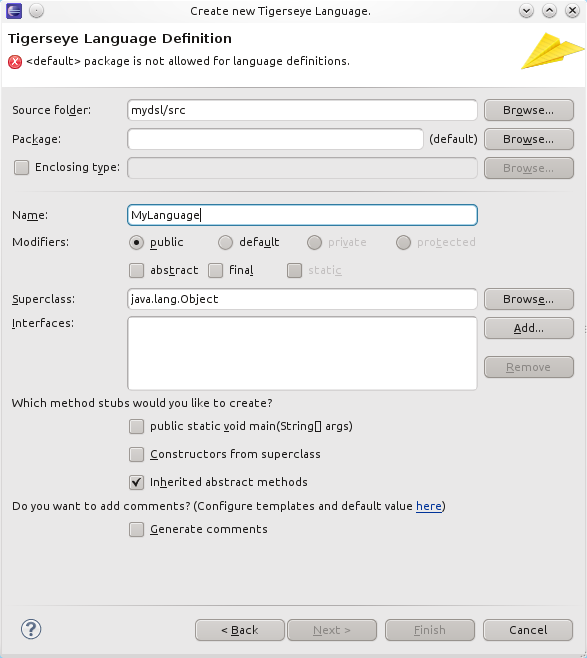
\includegraphics[width=.5\textwidth,keepaspectratio=true]{./pics/tigerseye_language_definition_page1.png}
	  \caption{Tigerseye Language Definition Wizard Page 1}
	  \label{fig:tiger_lang_definition_page1}
	\end{figure}
	
	\begin{figure}
	  \centering
	  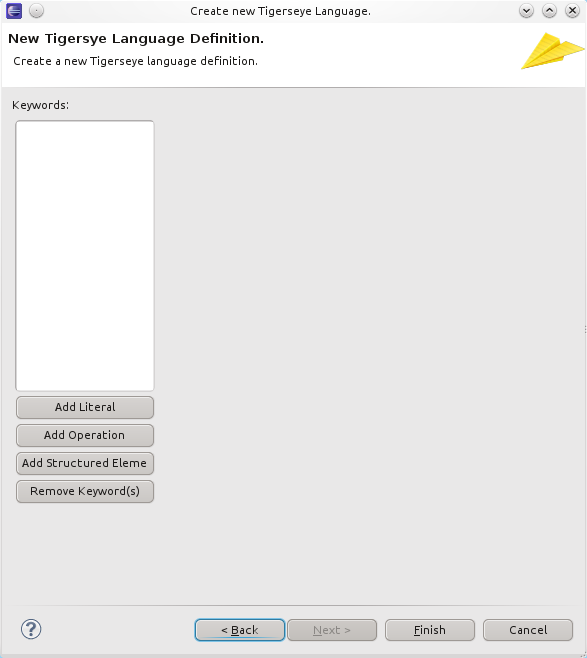
\includegraphics[width=.5\textwidth,keepaspectratio=true]{./pics/tigerseye_language_definition_page2.png}
	  \caption{Tigerseye Language Definition Wizard Page 2}
	  \label{fig:tiger_lang_definition_page2}
	\end{figure}
	
	\subsection{New \tiger Class Wizard}
	  The new \emph{\tiger Class Wizard} enables easy creation of new DSL classes. In Figure \ref{fig:new_tiger_class_page} the Wizard is shown. It is basically an adjusted version of the new Java Class Wizard. Additionally to being able to define the typical class properties a DSL can be chosen which one wishes to use in the class.

	\begin{figure}
	  \centering
	  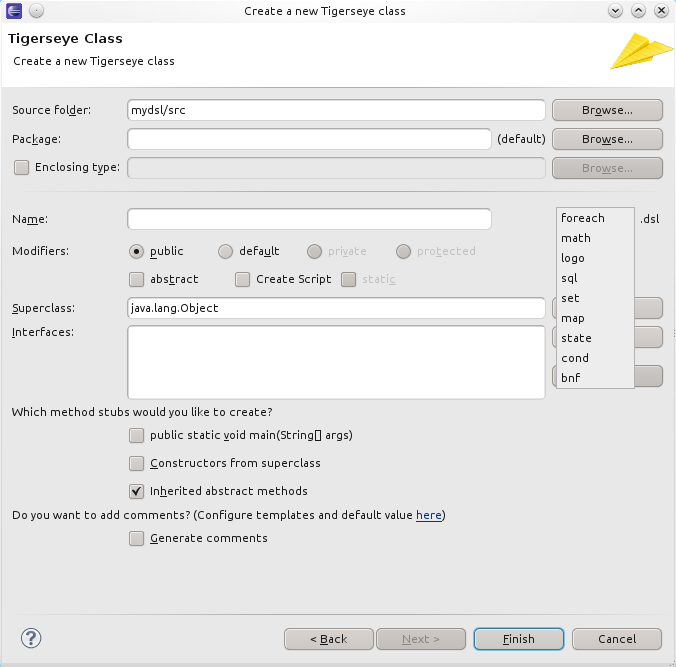
\includegraphics[scale=.5]{./pics/new_tigerseye_class_wizard.png}
	  \caption{New Tigerseye Class Wizard}
	  \label{fig:new_tiger_class_page}
	\end{figure}	
	
	
	\subsection{Launch Tigerseye DSL}
	  A \tiger1 DSL can be launched using the launch shortcut or via the \textit{Run Configurations} dialog. Figure \ref{fig:launch_shortcut} shows a launch using a launch shortcut. Figure  \ref{fig:launch_run_configurations_dialog} shows the launch via the \emph{Run Configurations Dialog}. There a new launch can be configured or a previous launch adjusted. On the \emph{Tigerseye} tab the project from which a DSL will be launched as well as the dsl file to launch can be chosen. When using the launch shortcut the Groovy default launch configuration is assumed which will set additional classpath properties. Later these can be modified using this dialog.
	
	\begin{figure}
	  \centering
	  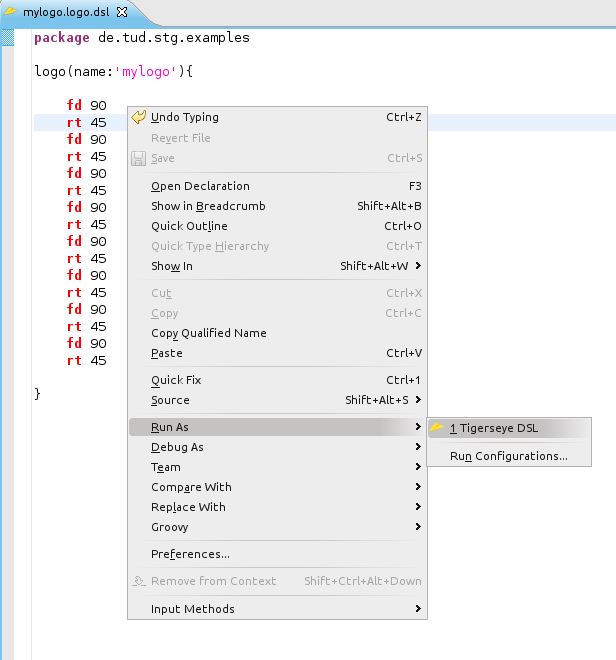
\includegraphics[scale=0.5]{./pics/launch_shortcut.png}
	  \caption{Launch via Context Menu}
	  \label{fig:launch_shortcut}
	\end{figure}

	\begin{figure}
	  \centering
	  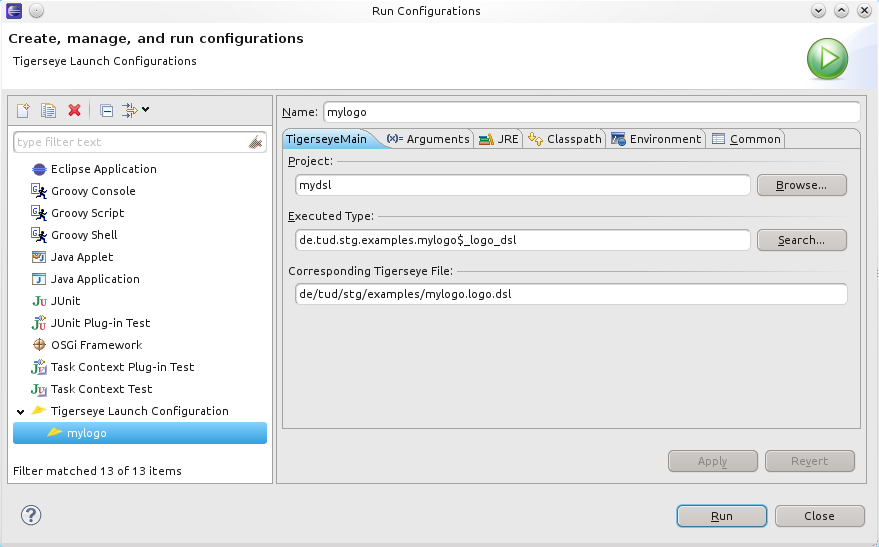
\includegraphics[scale=.5]{./pics/launch_run_configurations_dialog.png}
	  \caption{Launch via the Run Configurations Dialog}
	  \label{fig:launch_run_configurations_dialog}
	\end{figure}

  \section{Examples}\label{sec:examples}
	This section showcases typical use cases for the \tiger IDE. 
	
	\subsection{Creating a new \tiger Language Definition}
	
	The usage of the \emph{New Tigerseye Language Definition} wizard will be explained by creating a \emph{Trivalent-DSL}. A
	Trivalent logic DSL adds an \texttt{unknown (U)} value to the boolean values \texttt{true (T)} and \texttt{false (F)}, so \texttt{T\&U} is U and \texttt{T|U} is T and so on.
	
	\begin{itemize}
	 \item First create a new Java Project. This Project will contain the Trivalent language created by the wizard. In this example a project called \texttt{de.tud.stg.tigerseye.examples.trivalent} will be created
	 \item Right Click on the Project and choose \emph{New > Other}.
	 \item Choose \emph{Tigerseye Language Definition} in the \emph{Tigerseye} folder (Figure \ref{fig:new_tiger_lang}).
	 \item Each language definition consists of a Groovy class that defines all operations, literals and structured elements of the DSL. Type \texttt{TrivalentDSL} as the class name, \texttt{de.tud.stg.tigerseye.examples.trivalent} as the package and select \emph{Next} (Figure \ref{fig:example_newlang_newlangclass}).
	 \item Now add three new literals: \texttt{T} (true), \texttt{F} (false) and \texttt{U} (unknown). They are all of type Trivalent (Figure \ref{fig:example_newlang_literalsadded}). After finishing the wizard these three classes and the supertype Trivalent will be created. Notice that T, F and U extend Trivalent.
	\item The only operation will be an enhanced println which takes a String and a Trivalent expression and prints both, e.g. \texttt{puts("T|U: ",T|U)} will produce \texttt{T|U: T}. The return type should be \texttt{void} so we just let the \texttt{Return type:} field empty. For each operation you can choose if setting a breakpoint on a line containing this keyword should be possible (Figure \ref{fig:example_newlang_operationadded}). Also you can define all parameters and their types.
	\item Now add a repeat-statement. The following will simply print \texttt{T: T} ten times to stdout.
	  \begin{verbatim}	  
repeat(10) {
  puts("T:",T);
}
	  \end{verbatim}
	The return type will be \texttt{void} and there is one parameter named \texttt{n}. Select \texttt{explicit parameters} (Figure \ref{fig:example_newlang_structuredelementadded}).
	Again, you can choose if it should be possible to set a breakpoint on a line containing this keyword.
	\item After you select \texttt{Finish} a dialog will pop up asking you if you want to add the \tiger runtime libraries (Figure \ref{fig:example_newlang_addruntime}). Usually you should say yes, since language definitions have dependencies to the runtime libraries.
	\item The final result is shown in Figure \ref{fig:example_newlang_generatedcode}. For the new type \texttt{Trivalent} as well as for the literals \texttt{T,U and F} a separate Groovy class is created. The language configuration is defined in the \texttt{TrivalentDSL} class.
	\end{itemize}

	\begin{figure}
	  \centering
	  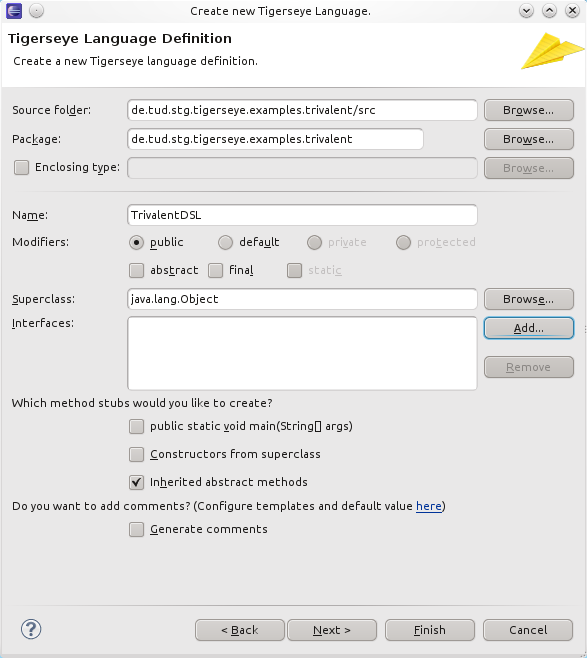
\includegraphics[scale=.5,keepaspectratio=true]{./pics/example_newlang_newlangclass.png}
	  \caption{New TrivalentDSL Language Defintion}\label{fig:example_newlang_newlangclass}
	\end{figure}

	\begin{figure}
	  \centering
	  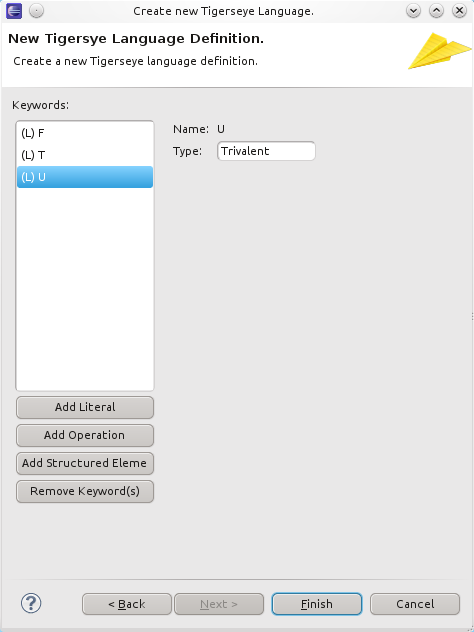
\includegraphics[scale=.5,keepaspectratio=true]{./pics/example_newlang_literalsadded.png}
	  \caption{TrivalentDSL Language Definition with Literals added}\label{fig:example_newlang_literalsadded}
	\end{figure}
	
	\begin{figure}
	  \centering
	  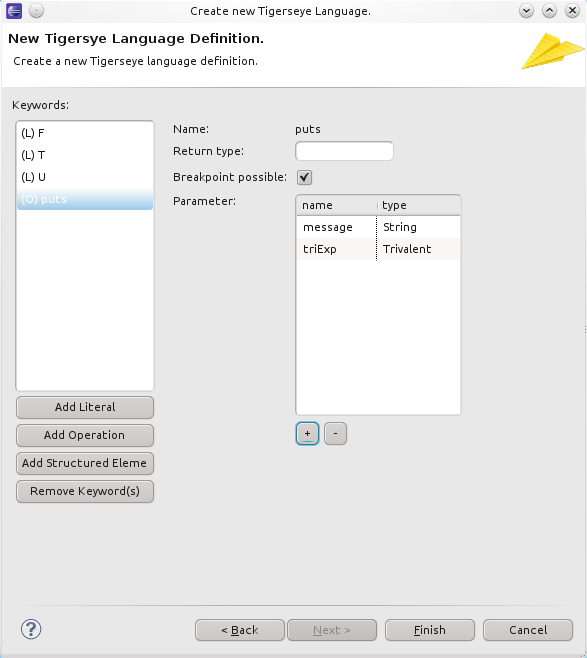
\includegraphics[scale=.5,keepaspectratio=true]{./pics/example_newlang_operationadded.png}
	  \caption{TrivalentDSL Language Definition Operation \texttt{puts} added}\label{fig:example_newlang_operationadded}
	\end{figure}
	
	\begin{figure}
	  \centering
	  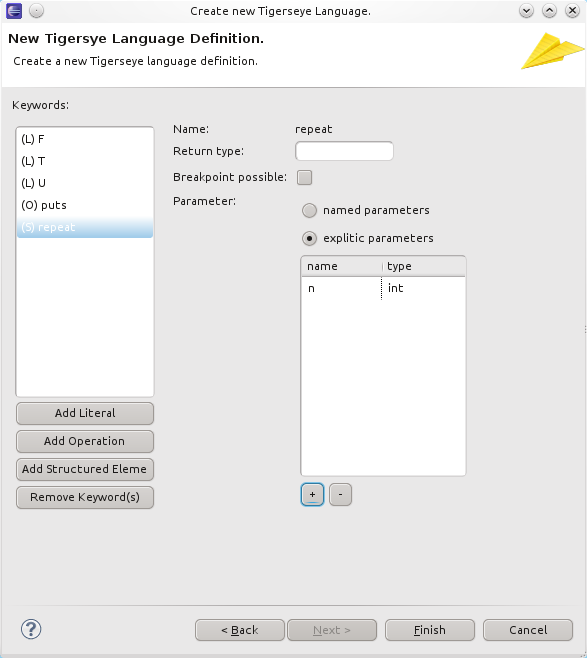
\includegraphics[scale=.5,keepaspectratio=true]{./pics/example_newlang_structuredelementadded.png}
	  \caption{TrivalentDSL Language Definition Structured Element \texttt{repeat} added}\label{fig:example_newlang_structuredelementadded}
	\end{figure}
	
	\begin{figure}
	  \centering
	  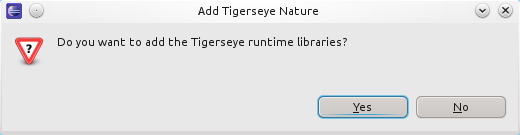
\includegraphics[scale=.5,keepaspectratio=true]{./pics/example_newlang_addruntime.png}
	  \caption{Question Dialog to add \tiger Runtime Libraries}\label{fig:example_newlang_addruntime}
	\end{figure}

	\begin{figure}
	  \centering
	  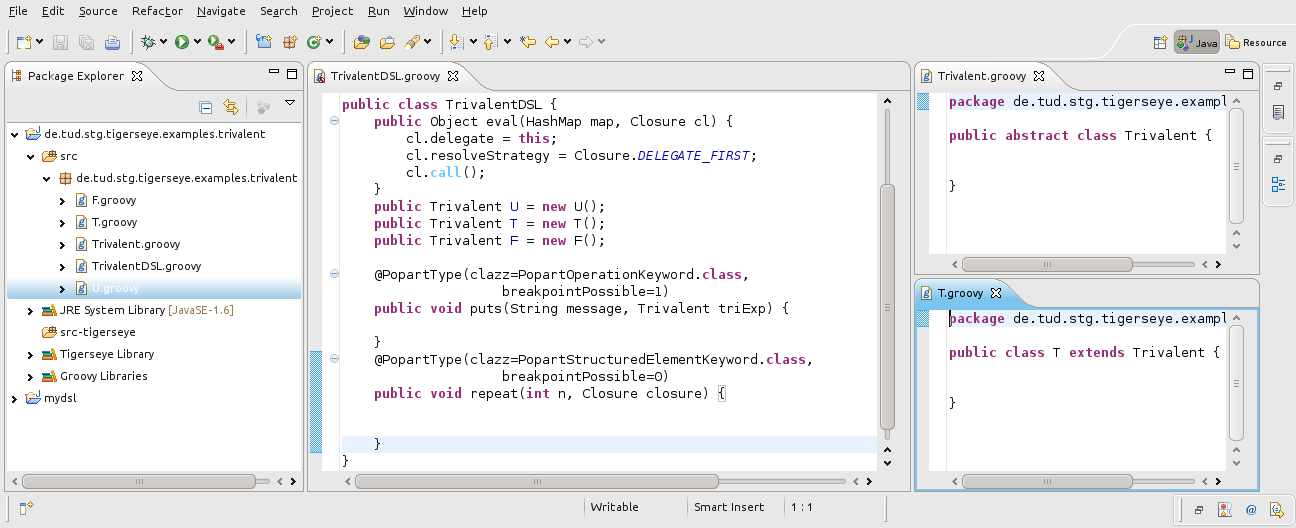
\includegraphics[scale=.5,keepaspectratio=true]{./pics/example_newlang_generatedcode.png}
	  \caption{TrivalentDSL Generated Classes and Code}\label{fig:example_newlang_generatedcode}
	\end{figure}

  \subsection{Deployment of a \tiger Language}
  
  To deploy a new language s.t., the user converts his designed language to a plug-in project. This plug-in project will declare its dependencies to two \tiger plug-ins:
  \begin{itemize}
   \item \texttt{de.tud.stg.tigerseye}
   \item \texttt{de.tud.stg.tigerseye.eclipse.core}
  \end{itemize}
  The \texttt{de.tud.stg.tigerseye} plug-in provides the dependent on libraries and the \texttt{de.tud.stg.tigerseye.eclipse.core} plug-in the extension which declares that this plug-in project actually provides a new language.
  
  The following steps have to be performed:
  \begin{enumerate}
   \item Convert the language definition project to a plug-in project. (Figure \ref{fig:example_deploy_converttoplugin})
   \item In the \texttt{MANIFEST.MF} file add the dependencies to the two Tigerseye plug-ins. (Figure \ref{fig:example_deploy_addplugindependencies})
   \item Now open the \texttt{plugin.xml} and go the \texttt{Extensions} tab. Add the \texttt{de.tud.stg.tigerseye.dslDefinitions} extension point. On the extension point select \texttt{New > language}. There you can define the language class to be used. In this example this would be \texttt{de.tud.stg.tigerseye.examples.trivalent.Trivalent}. Additionally you should define a user friendly name of your new language, e.g. \emph{Trivalent DSL}. Optionally you can define the default extension identifying your language, such as \texttt{tri}. Figure \ref{fig:example_deploy_extensionpoint} shows the example configuration. The extension can also be configured using the \tiger preference pages.
   \item Currently only the deployment for development is supported. Language can either be copied or linked inside the eclipse instance in which the \tiger plug-in is developed. The next time the \tiger Eclipse instance is started the language will be visible in the preference pages and can be used.
%    \item Now you can use the export functionality to export the language as a plug-in into a separate jar-file. This can then be copied either into Eclipse's \texttt{dropins} folder or into the \texttt{plugins} folder.
%    \item After a final restart the language should be visible in the languages preference page.
  \end{enumerate}

  	\begin{figure}
	  \centering
	  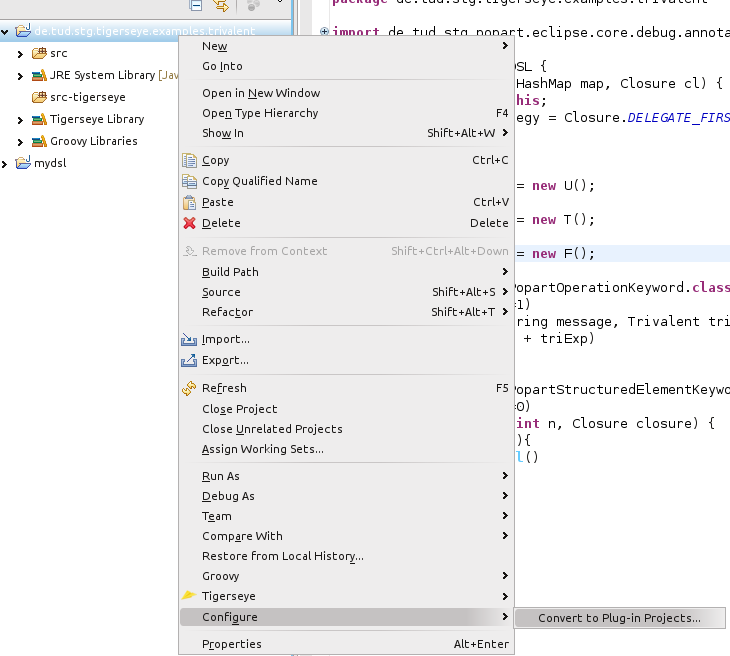
\includegraphics[scale=.5,keepaspectratio=true]{./pics/example_deploy_converttoplugin.png}
	  \caption{Add Plug-in Project Nature}\label{fig:example_deploy_converttoplugin}
	\end{figure}
	 
	\begin{figure}
	  \centering
	  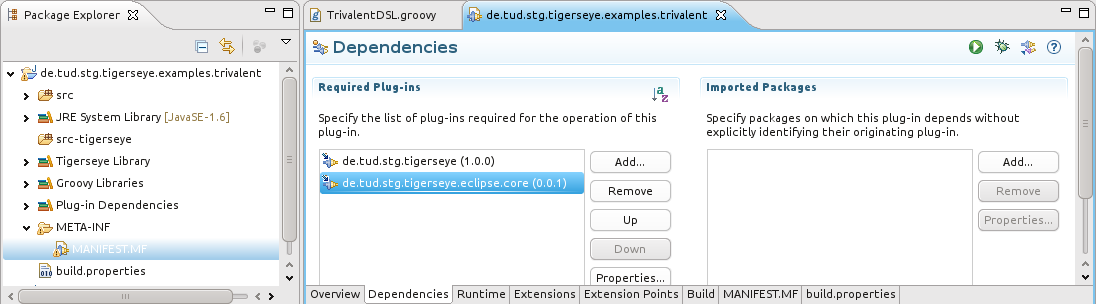
\includegraphics[scale=.5,keepaspectratio=true]{./pics/example_deploy_addplugindependencies.png}
	  \caption{Add Plug-in Depedencies to \tiger}\label{fig:example_deploy_addplugindependencies}
	\end{figure}
	
		\begin{figure}
	  \centering
	  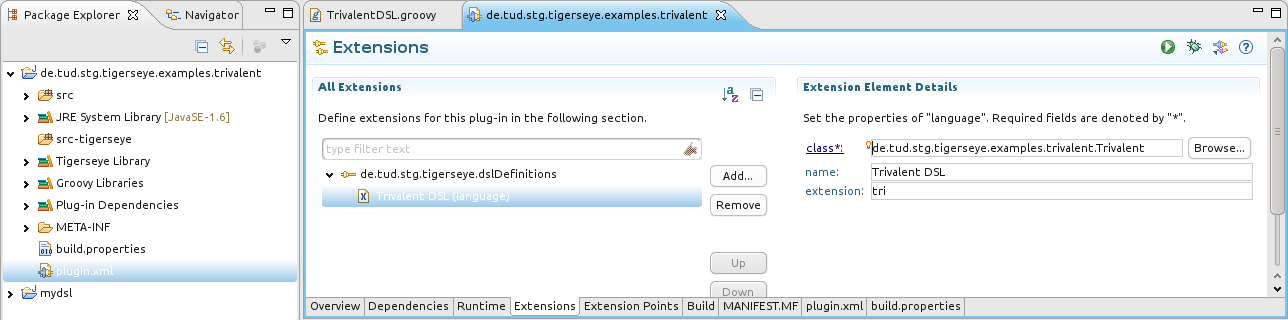
\includegraphics[scale=.5,keepaspectratio=true]{./pics/example_deploy_extensionpoint.png}
	  \caption{\texttt{dslDefinitions} Extension Point Configuration}\label{fig:example_deploy_extensionpoint}
	\end{figure}

  
  popartLanguage extension point so that the core of
generic POPART plug-in can find the DSL interpreter class file.
The use has to perform the following steps:
1.Create a new PDE Plug-in project for the language:
1.„New > Project > Other … Plug-in from existing JAR archive“

	

  \listoftables
  \listoffigures\addcontentsline{toc}{section}{\listfigurename}
\end{document}
